% !TeX spellcheck = <none>
%===============METODOLOGÍA==================
\section{Metodología}
Para la realización del trabajo terminal se seguirá la metodología descrita por el Modelo en Cascada El modelo de la cascada, a veces llamado ciclo de vida clásico, sugiere un enfoque sistemático y secuencial para el desarrollo del software, que comienza con la especificación de los requerimientos por parte del cliente y avanza a través de planeación, modelado, construcción y despliegue, para concluir con el apoyo del software terminado. \cite{MetodoCascada} \\

En la Figura \ref{fig:IntroduccionMetodologiaC} se muestran las actividades abordadas por el modelo en Cascada.

\begin{figure}[htbp!]
	\centering
	\fbox{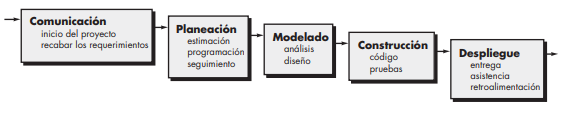
\includegraphics[width=\textwidth]{DisenoEstructura/imagenes/modelo-en-cascada}}
	\caption{Fases del Modelo en Cascada}
	\label{fig:IntroduccionMetodologiaC}
\end{figure}
\newpage

El desarrollo se llevará a cabo de la siguiente manera: \\

 \begin{itemize}
 	\item \textbf{Comunicación}: En este punto definiremos los requerimientos del sistema. (Protocolo)
 	\item \textbf{Planeación}: Con base en los requerimientos se estimará y en caso de necesitar modificaciones en alcance se definirán los nuevos requerimientos.
 	\item \textbf{Modelado}: Se modelarán los requerimientos viables con base en la estimación.
 	\item \textbf{Construcción}: Se desarrollaran los requerimientos definidos y se realizarán pruebas, es qui donde se plantea la implmentación de SCRUM.
 	\item \textbf{Despliegue}: Se entrega el desarrollo con pruebas documentación y mejoras. 
 \end{itemize}

Además del Modelo en Cascada, este trabajo terminal utilizará SCRUM como marco de referencia para el desarrollo de la aplicación, ya que los principios Scrum son congruentes con el manifiesto ágil y se utilizan para guiar actividades de desarrollo dentro de un proceso de análisis que incorpora las siguientes actividades estructurales: requerimientos, análisis, diseño, evolución y entrega \cite{MetodoCascada}. Como se plantea utilizar cascada hasta el punto de \textbf{modelado}, la implementación de SCRUM será viable ya que por su definición solo tendrá que organizar e implementar el desarrollo con este marco de referencia.

\begin{figure}[htbp!]
	\centering
	\fbox{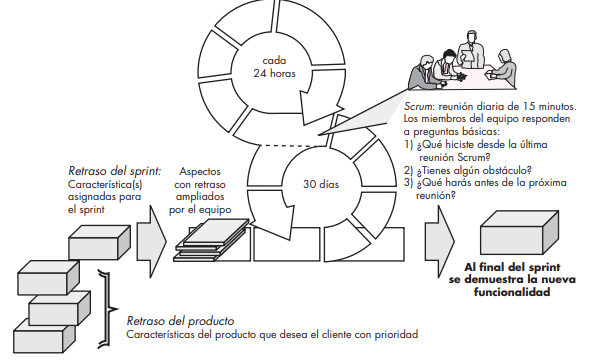
\includegraphics[width=\textwidth]{DisenoEstructura/imagenes/SCRUM}}
	\caption{SCRUM}
	\label{fig:IntroduccionMetodologiaS}
\end{figure}
\newpage